\documentclass[12pt]{article}
\usepackage{enumitem}

\usepackage[left=25mm, right=25mm, top=25mm, bottom=25mm, headheight=25mm]{geometry}
\usepackage{graphicx} % Required for inserting images
\usepackage{subfig} % Poder colocar más de una imagen en una {Figura}
\usepackage[figurename=Imagen]{caption} % Cambiar la descripción de la Image 
\usepackage[utf8]{inputenc} % Idioma español
\usepackage[spanish]{babel} % Idioma español

% Para poder ajustar los colores en las referencias que se hagan
\usepackage{hyperref}
\hypersetup{
    colorlinks=true,
    linkcolor = black,
    citecolor = blue,
    urlcolor = blue
}

% Dar formato a las páginas y colocar el \rfoot{De forma que nos interese}
\usepackage{parskip}
\usepackage{lastpage}
\usepackage{xcolor}
\usepackage{fancyhdr}
\pagestyle{fancy}
\cfoot{}
\rfoot{Página \thepage\ de \pageref{LastPage}}
\rhead{}
\lhead{}
\renewcommand{\headrulewidth}{0pt}

% Parámetros que pueden cambiar ----------------------------------------------------------------------------
% Nombres
\newcommand{\Profesor}{Profesor: Edgar Tista García}
\newcommand{\Materia}{Asignatura: Estructura de Datos y Algoritmos II}
\newcommand{\Grupo}{Grupo:  5}
\newcommand{\Nombre}{Integrantes:  Giron Escalona Erendira Nayely, López Martínez Diana , Zarate Menes Quetzalli}
\newcommand{\NoLista}{No. de lista: 12, 20, 35}
\newcommand{\Proyecto}{PROYECTO \#1 - COMPLEJIDAD COMPUTACIONAL EN LOS ALGORITMOS DE ORDENAMIENTO}
\newcommand{\Semestre}{Semestre: 2024-2}
\newcommand{\Fecha}{Fecha de entrega: 24 de marzo del 2024}
\newcommand{\Observaciones}{Observaciones:}
\newcommand{\Calificacion}{CALIFICACIÓN:}

\newcommand{\TituloP}{TRABAJO ESCRITO DEL PROYECTO }
\newcommand{\Titulo}{\Proyecto\\\TituloP}


\begin{document}
\begin{center}
    \LARGE\textbf{\TituloP}\par\vspace{0.7cm}
\end{center}
\Large{\Proyecto}\par\vspace{0.6cm}
\Large{\Profesor}\par\vspace{0.6cm}
\Large{\Materia}\par\vspace{0.6cm}
\Large{\Grupo}\par\vspace{0.6cm}
\Large{\Nombre}\par\vspace{0.6cm}
\Large{\NoLista}\par\vspace{0.6cm}
\Large{\Semestre}\par\vspace{0.6cm}
\Large{\Fecha}\par\vspace{0.6cm}
\Large{\Observaciones}\par\vspace{0.6cm}

\begin{center}
    \Large{\Calificacion}\par\vspace{0.6cm}
\end{center}
% -------------------------------------------------------- Empieza el desarrollo de la práctica

\newpage
\textcolor{blue}{\textbf{OBJETIVO}}
\par\vspace{0.4cm}
Que el alumno observe la complejidad computacional de los algoritmos de ordenamiento para
comparar su eficiencia de ejecución en grandes volúmenes de información
\par\vspace{1.5cm}
\textcolor{blue}{\textbf{INTRODUCCIÓN}}
\par\vspace{0.4cm}
En nuestro proyecto, abordamos el estudio teórico y práctico de los algoritmos de ordenamiento, fundamentales en el campo de la ciencia de la computación. Estos algoritmos son esenciales para la organización y manejo eficiente de datos, una habilidad clave en la era de la información.
\par\vspace{0.4cm}
InsertionSort es un algoritmo intuitivo que construye la salida ordenada elemento por elemento, insertando cada nuevo elemento en su posición correcta dentro de la parte ya ordenada.
\par\vspace{0.4cm}
SelectionSort mejora este proceso seleccionando el elemento más pequeño de la parte no ordenada y colocándolo al principio de la lista ordenada.
\par\vspace{0.4cm}
Heapsort transforma la lista en un montículo binario y luego extrae los elementos de manera ordenada, aprovechando la estructura de árbol para mejorar el tiempo de ejecución.
\par\vspace{0.4cm}
Bubblesort es un método simple que revisa repetidamente la lista para intercambiar elementos adyacentes que están en el orden incorrecto.
\par\vspace{0.4cm}
Quicksort divide la lista en dos partes, ordenando cada una de ellas de manera independiente a través de un proceso recursivo basado en un pivote.
\par\vspace{0.4cm}
Mergesort también utiliza la recursividad, dividiendo la lista en mitades hasta llegar a listas de un solo elemento y luego combinándolas de manera ordenada.
\par\vspace{0.4cm}
Finalmente, exploraremos un algoritmo adicional, que seleccionaremos por su relevancia y eficacia comparativa, para ampliar nuestra comprensión de estas técnicas de ordenamiento.
\par\vspace{0.4cm}
Nuestro análisis se centrará en cómo estos algoritmos manejan el incremento en el tamaño de los datos, observando la cantidad de operaciones necesarias para alcanzar la lista ordenada final. Este enfoque nos permitirá no solo entender los principios básicos de funcionamiento de cada algoritmo, sino también su comportamiento y rendimiento en condiciones reales y variadas.
\par\vspace{1.5cm}
\textcolor{blue}{\textbf{DESARROLLO}}
\par\vspace{0.4cm}
\textcolor[rgb]{0.13, 0.55, 0.13}{\textbf{Menu Principal}}
\par\vspace{0.4cm}
En relación al requisito de manejar diferentes tamaños de arreglos, se ha implementado una función denominada “llenarArregloConAleatorios”. En esta función, se utiliza la clase Random que se encuentra en el paquete java.util.
\par\vspace{0.4cm}
Consideraciones para Inicializar Arreglos
\par\vspace{0.4cm}
En el contexto de la inicialización de arreglos, nos encontramos con un desafío importante: ¿cómo manejar diferentes tamaños de arreglos de manera eficiente y efectiva? Durante nuestras discusiones, evaluamos diversas alternativas y llegamos a una solución que equilibra la funcionalidad con las limitaciones de recursos.
\par\vspace{0.4cm}
\begin{enumerate}
    \item Ciclo de for para Tamaños de Arreglo:
          \begin{itemize}
              \item Inicialmente, consideramos la posibilidad de utilizar un ciclo iterativo para recorrer una gama de tamaños de arreglo. Esto nos permitiría mostrar los resultados en pantalla y evaluar la complejidad del algoritmo para cada tamaño.
              \item Sin embargo, surgió una preocupación importante: ¿qué sucede si la computadora del usuario no puede manejar un arreglo excesivamente grande? La ejecución podría volverse ineficiente o incluso agotar los recursos disponibles.
          \end{itemize}
    \item Solución: Menú de Elección de Tamaño:
          \begin{itemize}
              \item Para abordar esta preocupación, optamos por implementar un menú interactivo. En lugar de asumir un tamaño de arreglo predeterminado, le damos al usuario la capacidad de elegir el tamaño deseado.
              \item El menú permite al usuario especificar el número de elementos en el arreglo. Esto garantiza que la prueba de complejidad se realice dentro de los límites de capacidad de su máquina.
          \end{itemize}
    \item Función con Parámetro de Tamaño:
          \begin{itemize}
              \item Para llevar a cabo esta implementación, creamos una función llamada “llenarArregloConAleatorios”. Dentro de este menú, se le pasa como parámetro el tamaño de arreglo deseado.
              \item La función utiliza la clase Random del paquete java.util para generar valores aleatorios y llenar el arreglo con datos representativos.
          \end{itemize}
\end{enumerate}
\par\vspace{0.4cm}
Consideraciones para Comparar Complejidades de Algoritmos de Ordenamiento.
\par\vspace{0.4cm}
En nuestro análisis riguroso de los algoritmos de ordenamiento, nos encontramos con un desafío fundamental: ¿cómo comparar de manera justa las complejidades de diferentes métodos en un escenario realista? Para abordar esta cuestión, diseñamos una estrategia que garantiza una evaluación imparcial y significativa.
\par\vspace{0.4cm}
\begin{enumerate}
    \item El Dilema del Mejor Caso:
          \begin{itemize}
              \item Al comparar algoritmos, es crucial considerar el mejor caso, el peor caso y el caso promedio.
              \item Siempre que enviáramos un arreglo ya ordenado a un nuevo método de ordenamiento, estaríamos en el mejor caso. Sin embargo, esto no reflejaría la realidad, ya que en situaciones reales, rara vez se reciben arreglos perfectamente ordenados.
          \end{itemize}
    \item Solución: Arreglos Desordenados y Copias:
          \begin{itemize}
              \item Para abordar este sesgo, creamos dos copias del mismo arreglo:
                    \begin{itemize}
                        \item Arreglo A (Original): Generado aleatoriamente con valores desordenados.
                        \item Arreglo B (Copia): Inicialmente idéntico a A, pero se le asignará el resultado de un algoritmo de ordenamiento.
                    \end{itemize}
              \item Ejecutamos cada algoritmo de ordenamiento en B, lo que garantiza que estemos evaluando el caso promedio.
          \end{itemize}
    \item Repetibilidad y Tamaño del Arreglo:
          \begin{itemize}
              \item El usuario selecciona el tamaño del arreglo en el menú interactivo.
              \item Al repetir el proceso con el mismo arreglo desordenado, aseguramos la consistencia y la comparabilidad.
          \end{itemize}
\end{enumerate}
\par\vspace{0.4cm}
En resumen, nuestra metodología garantiza un análisis imparcial y realista de los algoritmos de ordenamiento. Al utilizar arreglos desordenados y copias, evitamos el sesgo del mejor caso y obtenemos una visión más precisa de la eficiencia de cada método.

\textcolor[rgb]{0.13, 0.55, 0.13}{\textbf{InsertionSort}}
\par\vspace{0.4cm}
En la optimización del algoritmo \textit{InsertionSort}, se introdujeron contadores para monitorear las operaciones de inserción, intercambio y comparación. Estos contadores son cruciales para analizar la complejidad del algoritmo, ya que proporcionan una cuantificación directa de las operaciones elementales que realiza.

Para integrar estos contadores, se realizaron las siguientes modificaciones en el código:

\begin{itemize}
    \item En la estructura \texttt{while}, que evalúa si el índice \texttt{j} es mayor o igual a cero y si el elemento en la posición \texttt{j} es mayor que el valor en el índice \texttt{index}, se incrementa el contador de comparaciones. Esto se debe a que en cada iteración de esta estructura se realiza una comparación.
    \item Si la condición de comparación es verdadera, se procede a intercambiar los valores del arreglo en las posiciones \texttt{j+1} y \texttt{j}. En este punto, se incrementa el contador de intercambios, reflejando la realización de esta operación.
    \item La última modificación consistió en añadir el contador de inserciones, el cual se incrementa después de la estructura \texttt{while}. Esto indica que se ha encontrado la posición final para el valor que se está insertando, y por lo tanto, se contabiliza una inserción.
\end{itemize}

La implementación de estos contadores no presentó dificultades significativas, debido a la simplicidad inherente al algoritmo de \textit{InsertionSort}. La adición de estas métricas permite un análisis más detallado y preciso de la complejidad del algoritmo, facilitando la comprensión de su comportamiento y eficiencia en diferentes escenarios de ordenamiento.

\textcolor[rgb]{0.13, 0.55, 0.13}{\textbf{SelectionSort}}
\par\vspace{0.4cm}
\section*{Algoritmo de Selection Sort}
\par\vspace{0.4cm}
El algoritmo de \textbf{Selection Sort} sigue un enfoque simple y directo para ordenar una lista de elementos. Funciona de la siguiente manera:
\par\vspace{0.4cm}
\begin{enumerate}
    \item Encuentra el elemento más pequeño en la lista.
    \item Intercambia el elemento más pequeño con el primer elemento.
    \item Busca el siguiente elemento más pequeño y lo intercambia con el segundo elemento.
    \item Repite el proceso hasta que todos los elementos estén ordenados.
\end{enumerate}
\par\vspace{0.4cm}
Este algoritmo divide el conjunto de elementos en dos partes: la parte ordenada (izquierda) y la parte no ordenada (derecha). En cada iteración, busca el elemento más pequeño en la parte no ordenada y lo coloca en su posición correcta en la parte ordenada. A pesar de su simplicidad, \textbf{Selection Sort} puede ser ineficiente para grandes conjuntos de datos debido a su complejidad cuadrática.
\par\vspace{0.4cm}
\subsection*{Funcionalidad de la Clase Selection Sort}
\par\vspace{0.4cm}
La clase \textbf{Selection Sort} contiene el método \texttt{selection}, que toma un arreglo de enteros como entrada y representa la implementación del algoritmo. La funcionalidad se describe a continuación:
\begin{itemize}
    \item Inicializa tres variables para llevar un registro del número de iteraciones, comparaciones e intercambios realizados durante el proceso de ordenamiento.
    \item Obtiene la longitud del arreglo para determinar el número de elementos a ordenar.
    \item Establece un bucle exterior que se ejecuta para cada elemento del arreglo, excepto el último.
    \item Dentro del bucle, incrementa el contador de iteraciones.
    \item Inicializa la variable \texttt{min} con el índice actual del bucle exterior.
    \item Ejecuta un bucle interior para cada elemento restante en el arreglo.
    \item Incrementa el contador de comparaciones cada vez que se compara un elemento.
    \item Si encuentra un elemento menor, actualiza la posición del mínimo.
    \item Intercambia el mínimo elemento encontrado con el primer elemento de la parte no ordenada.
    \item Incrementa el contador de intercambios al realizar un intercambio de elementos.
    \item Cierra los ciclos y presenta los resultados utilizando la función \texttt{printArray}.
\end{itemize}
\par\vspace{0.4cm}
Las modificaciones realizadas al algoritmo de \textbf{Selection Sort} han agregado contadores para registrar el número de \textit{iteraciones}, \textit{comparaciones} e \textit{intercambios} realizados durante el proceso de ordenamiento. Estos contadores se han incorporado en bucles adecuados dentro del algoritmo. La variable \textit{itera} se incrementa en cada iteración del bucle externo, \textit{comp} se incrementa cada vez que se realiza una comparación entre elementos, y \textit{swaps} se incrementa cada vez que se realiza un intercambio de elementos. Estos contadores proporcionan una forma de medir el rendimiento del algoritmo y entender mejor su comportamiento en diferentes conjuntos de datos.
\par\vspace{0.6cm}
\textcolor[rgb]{0.13, 0.55, 0.13}{\textbf{HeapSort}}
\par\vspace{0.4cm}
En el desarrollo del algoritmo de ordenamiento por montículo (\textit{HeapSort}), se presentaron desafíos significativos para contabilizar las operaciones de comparación e intercambio. La complejidad radica en la naturaleza recursiva y la manipulación del arreglo durante la construcción y el ordenamiento del montículo.
\par\vspace{0.4cm}
Para abordar estas dificultades, se introdujeron dos contadores estáticos, \texttt{INTERCAMBIOS} y \texttt{COMPARACIONES}, que incrementan su valor en puntos estratégicos del algoritmo. En la función \texttt{heapifyASC}, se incrementa \texttt{COMPARACIONES} cada vez que se evalúa una condición para determinar el nodo más grande. Asimismo, \texttt{INTERCAMBIOS} se incrementa cada vez que se realiza un intercambio de elementos en el arreglo.
\par\vspace{0.4cm}
La contabilización de estas operaciones se realiza de esta forma debido a que proporciona una medida directa y clara del trabajo realizado por el algoritmo. Las comparaciones son indicativas de la cantidad de decisiones tomadas, mientras que los intercambios reflejan las modificaciones efectuadas sobre la estructura del montículo. Juntos, estos contadores ofrecen una visión integral del esfuerzo computacional requerido para ordenar el arreglo.
\par\vspace{0.4cm}
El método \texttt{imprimirContadores} se encarga de mostrar la suma de ambos contadores, ofreciendo así el número total de operaciones realizadas. Posteriormente, se reinician los contadores para evitar la acumulación de operaciones entre ejecuciones sucesivas del algoritmo.
\par\vspace{0.4cm}
En conclusión, el seguimiento de estas operaciones es fundamental para evaluar el rendimiento del algoritmo de \textit{HeapSort}, y los contadores implementados facilitan esta tarea de manera eficiente y sistemática.
\par\vspace{0.6cm}
\textcolor[rgb]{0.13, 0.55, 0.13}{\textbf{BubbleSort}}
\par\vspace{0.4cm}
El algoritmo de \textbf{Bubble Sort} cuenta con un enfoque simple y directo para ordenar una lista de elementos. Comienza comparando cada par de elementos adyacentes en la lista y los intercambia si están en el orden incorrecto. De esta manera, el elemento más grande "burbujea" hacia la parte superior de la lista en cada iteración. Este proceso se repite hasta que la lista esté completamente ordenada y ningún intercambio adicional sea necesario. Aunque es fácil de implementar y entender, \textbf{Bubble Sort} puede ser ineficiente para grandes conjuntos de datos debido a su complejidad cuadrática.
\par\vspace{0.4cm}
En cuanto a la funcionalidad, la clase \textbf{Bubble Sort} contiene lo siguiente:
\begin{itemize}
  \item El método \texttt{bubbleSort}, que toma un arreglo de enteros como parámetro y lo ordena utilizando el algoritmo \textbf{Bubble Sort}.
  \begin{itemize}
    \item Primero se obtiene la longitud del arreglo, lo que permite saber cuántos elementos hay que ordenar.
    \item Se inicializan tres variables para llevar un registro del número de iteraciones (\textit{iteraciones}), comparaciones (\textit{comparaciones}) e intercambios (\textit{intercambios}) realizados durante el proceso de ordenamiento.
    \item Se inicia un bucle externo que se encarga de iterar sobre cada elemento del arreglo, comenzando desde el último y avanzando hacia el primero.
    \item Dentro del bucle externo, se crea un segundo bucle para iterar sobre cada par de elementos adyacentes en el arreglo.
    \item Se establece una condición dentro del segundo bucle que verifica si el elemento actual es mayor que el siguiente en el arreglo.
    \item Si el elemento actual es mayor que el siguiente, se llama a la función \texttt{swap} para intercambiar los elementos y ordenarlos.
    \item Se cierran los ciclos y se presentan los resultados, auxiliándose de \texttt{printArray} para mostrar la lista antes y después de ordenar.
  \end{itemize}
\end{itemize}
Las modificaciones para el conteo de comparaciones en el algoritmo de \textbf{Bubble Sort} proporcionan una manera de evaluar y analizar su rendimiento. Al agregar contadores para estas operaciones, se puede monitorear cuántas veces se ejecuta cada paso crucial del algoritmo durante su ejecución. Esto permite cuantificar el rendimiento del algoritmo y compararlo con otros algoritmos de ordenamiento. Además, estas métricas ayudan a comprender mejor el comportamiento del algoritmo en diferentes conjuntos de datos y permiten identificar áreas para posibles mejoras o optimizaciones.
\par\vspace{0.6cm}
\textcolor[rgb]{0.13, 0.55, 0.13}{\textbf{QuickSort}}
\par\vspace{0.4cm}
La modificación principal fue agregar a los contadores las operaciones de comparaciones, intercambios e inserciones. Estas sirven para analizar la complejidad del algoritmo y compararlos con los otros algoritmos.
\par\vspace{0.4cm}
Para modificar el algoritmo y agregar estos contadores se realizó lo siguiente:
\begin{itemize}
    \item Dentro del método \texttt{partition} se agregan los contadores de las operaciones, para los intercambios, comparaciones e inserciones, los intercambios se implementan dentro del ciclo \texttt{for} después de haber verificado que el elemento en la posición $j$ del arreglo es decir el actual sea menor o igual al pivote se intercambian los elementos que se encuentran en las posiciones de los índices $i$ y $j$, se usó también al método \texttt{swap} el cual se encuentra en las utilerías y después de ello se usan los contadores de intercambios y comparaciones pues se están realizando ambas operaciones en este momento. Por último se agregó al contador de inserciones el cual se usó después de realizar la inserción del elemento usando el método \texttt{swap} el cual se encuentra en las utilerías. Ya que se debe incrementar cada que se realice esta operación.
\end{itemize}
\par\vspace{0.4cm}
La dificultad que se presentó fue que el número de los contadores se almacenaban conforme se utilizaba el algoritmo, para intentar solucionar esto creé un método para que reiniciara a los contadores y no se acumularan las operaciones. Sin embargo, esta no era la mejor solución, mi compañera Quetzalli me comentó que si se inicializan los contadores desde el principio en 0 no sería necesario reiniciarlos y desaparece el problema de acumulación de operaciones.
\par\vspace{0.6cm}
\textcolor[rgb]{0.13, 0.55, 0.13}{\textbf{MergeSort}}
\par\vspace{0.4cm}
Reflexiones sobre el Conteo de Operaciones en MergeSort
\par\vspace{0.4cm}
Durante mi análisis exhaustivo de los algoritmos de ordenamiento, me encontré con un desafío fundamental: ¿cómo comparar de manera justa las complejidades de diferentes métodos en un escenario realista? Permíteme compartir mis reflexiones al respecto:
\begin{enumerate}
    \item Dificultades Iniciales:
          \begin{itemize}
              \item Al evaluar la eficiencia de MergeSort, necesitaba una forma objetiva de medir su rendimiento.
              \item Contar las operaciones (comparaciones e inserciones) se convirtió en un aspecto crucial para evaluar su eficiencia.
          \end{itemize}
    \item Resolución: Conteo de Operaciones
          \begin{itemize}
              \item Introduje dos variables estáticas: INSERCIONES y COMPARACIONES.
              \item Cada vez que se realiza una comparación entre elementos del arreglo, incremento COMPARACIONES.
              \item Cada vez que se inserta un elemento en el arreglo auxiliar durante la fusión, incremento INSERCIONES.
          \end{itemize}
    \item Razón detrás del Conteo:
          \begin{itemize}
              \item Comparaciones: Representan la cantidad de veces que evaluamos si un elemento es mayor o menor que otro. Esto ayuda a medir la eficiencia en términos de decisiones tomadas.
              \item Inserciones: Representan la cantidad de veces que copiamos un elemento en el arreglo auxiliar durante la fusión. Esto refleja la cantidad de operaciones de escritura realizadas.
          \end{itemize}
    \item Uso en la Evaluación:
          \begin{itemize}
              \item Al imprimir los contadores al final de la ejecución, obtengo una visión completa del número total de operaciones realizadas.
              \item Esto me permite comparar MergeSort con otros algoritmos y evaluar su eficiencia en diferentes contextos.
          \end{itemize}
\end{enumerate}
\textcolor[rgb]{0.13, 0.55, 0.13}{\textbf{Adicional-CountingSort}}
\par\vspace{0.4cm}
\par\vspace{0.4cm}
Dificultades en el Conteo de Operaciones en Counting Sort
\par\vspace{0.4cm}
Como desarrollador, enfrenté varias dificultades al contar las operaciones realizadas en el algoritmo de ordenamiento por conteo (Counting Sort) que se presenta a continuación. A continuación, describo estas dificultades, cómo se resolvieron y por qué se contabilizan las operaciones de esa manera.
\par\vspace{0.4cm}
\begin{enumerate}
    \item \textbf{Bucles Anidados:}
          \begin{itemize}
              \item El código contiene varios bucles anidados, lo que dificulta contar con precisión las operaciones.
              \item El bucle más externo inicializa el arreglo de conteo, el segundo bucle cuenta la frecuencia de cada dígito y el tercer bucle reemplaza los elementos originales del arreglo según la frecuencia.
              \item Cada bucle contribuye al recuento total de operaciones, pero hacer un seguimiento de todas las iteraciones anidadas es complejo.
          \end{itemize}

    \item \textbf{Incremento de Contadores Dentro de Bucles:}
          \begin{itemize}
              \item Los contadores (INSERCIONES, ITERACIONES y COMPARACIONES) se incrementan dentro de los bucles.
              \item Por ejemplo, en la función findMax, los contadores se incrementan dentro del bucle que busca el valor máximo.
              \item Esto dificulta separar las operaciones relacionadas con cada tarea específica (por ejemplo, encontrar el valor máximo, contar frecuencias y reemplazar elementos).
          \end{itemize}

    \item \textbf{Operaciones Mixtas:}
          \begin{itemize}
              \item El código realiza diversas operaciones (asignaciones, comparaciones e incrementos) dentro de los mismos bucles.
              \item Por ejemplo, el bucle while dentro del tercer bucle realiza tanto asignaciones A[i++] = j como decrementos (count[j]--).
              \item Contar estas operaciones mixtas con precisión es complicado.
          \end{itemize}

    \item \textbf{Sentencias Condicionales:}
          \begin{itemize}
              \item El código incluye sentencias condicionales (por ejemplo, if (A[i] > max)) que afectan el recuento de operaciones.
              \item Estas condiciones conducen a diferentes caminos en el flujo de ejecución, lo que dificulta rastrear el número exacto de operaciones.
          \end{itemize}
\end{enumerate}
\par\vspace{0.4cm}
Resolución del Conteo
\par\vspace{0.4cm}
Para abordar estas dificultades, coloqué los contadores en puntos estratégicos del código:
\par\vspace{0.4cm}
\begin{itemize}
    \item \textbf{INSERCIONES}: Se incrementa al reemplazar elementos en el arreglo original.
    \item \textbf{ITERACIONES}: Se incrementa en bucles (tanto en bucles de inicialización como de conteo).
    \item \textbf{COMPARACIONES}: Se incrementa durante las comparaciones (por ejemplo, al encontrar el valor máximo).
\end{itemize}
\par\vspace{0.4cm}
El recuento final de operaciones se obtiene sumando estos tres contadores. Los métodos imprimirContadores y retornarContadores proporcionan el recuento total de operaciones.
\par\vspace{0.4cm}
Razón para Contar las Operaciones de Esta Manera
\par\vspace{0.4cm}
Los contadores elegidos (inserciones, iteraciones y comparaciones) representan operaciones comunes en algoritmos de ordenamiento:
\par\vspace{0.4cm}
\begin{itemize}
    \item Contar inserciones ayuda a rastrear cuántas veces se mueven los elementos.
    \item Contar iteraciones captura la complejidad general de los bucles.
    \item Contar comparaciones es esencial para comprender la eficiencia del algoritmo.
\end{itemize}
\par\vspace{0.4cm}
Al sumar estos contadores, obtenemos una visión completa del rendimiento del algoritmo.
\par\vspace{0.6cm}
\newpage
\textcolor{blue}{\textbf{IMPLEMENTACIÓN}}
\par\vspace{0.4cm}
\textbf{En cuanto a HeapSort, MergeSort y CountingSort}
EJECUCIONES: Para determinar el número de operaciones y el promedio de cada uno.
\par\vspace{0.4cm}
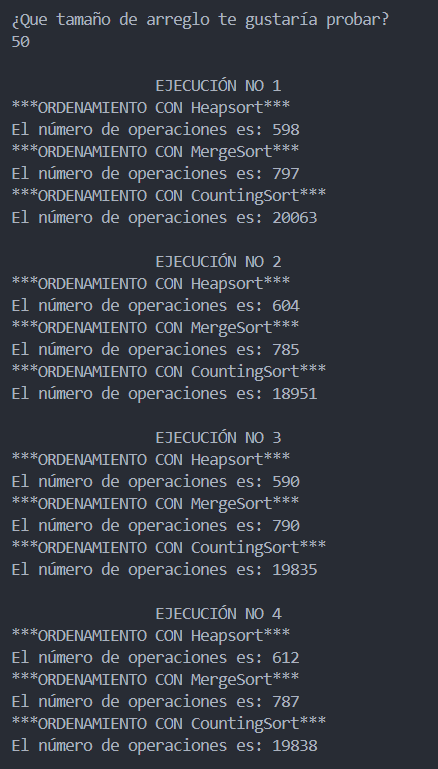
\includegraphics[width=7cm]{Images/Tam.50/1.png}
\par\vspace{0cm}
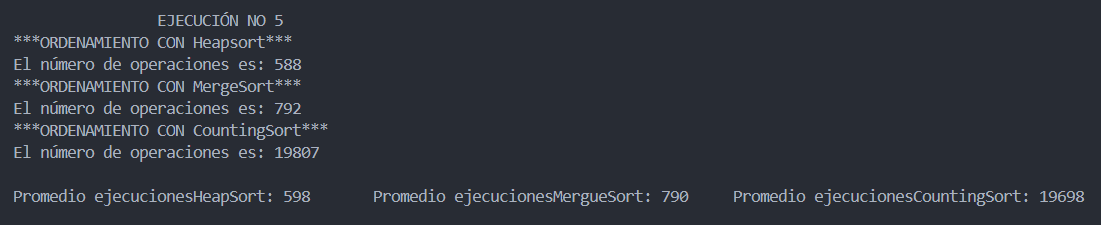
\includegraphics[width=16cm]{Images/Tam.50/2.png}
\newpage
\par\vspace{0.4cm}
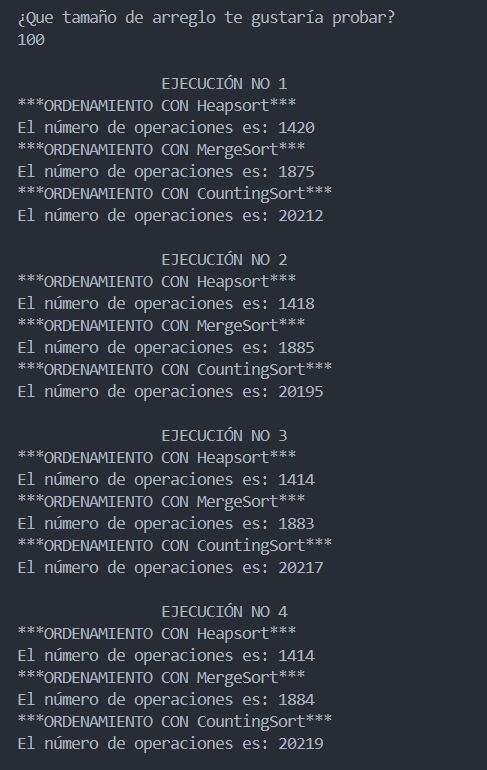
\includegraphics[width=9cm]{Images/Tam.100/1.png}
\par\vspace{0.4cm}
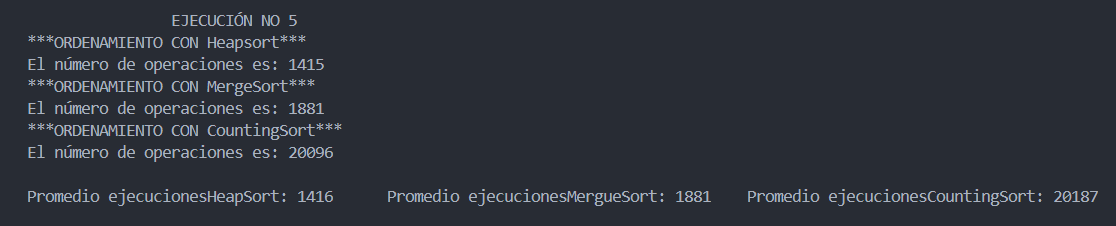
\includegraphics[width=16cm]{Images/Tam.100/2.png}
\par\vspace{0.4cm}
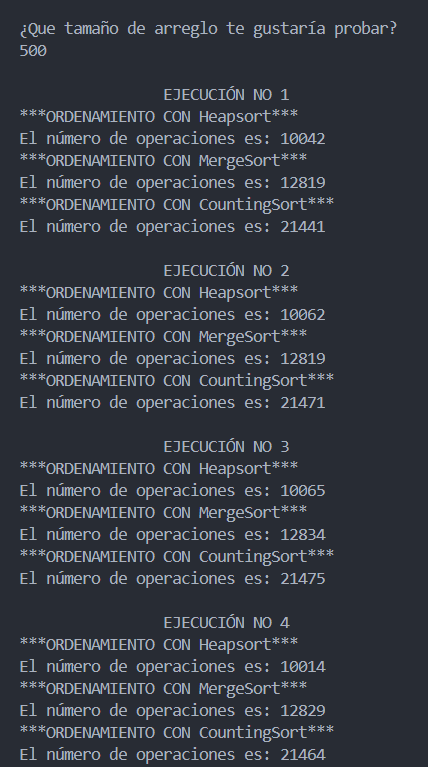
\includegraphics[width=9cm]{Images/Tam.500/1.png}
\par\vspace{0.4cm}
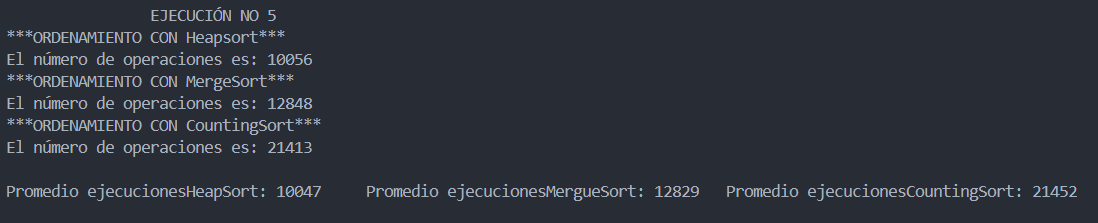
\includegraphics[width=16cm]{Images/Tam.500/2.png}
\par\vspace{0.4cm}
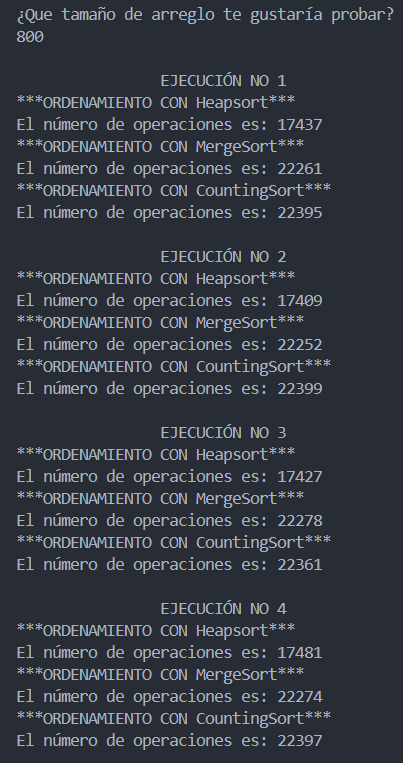
\includegraphics[width=9cm]{Images/Tam.800/1.png}
\par\vspace{0.4cm}
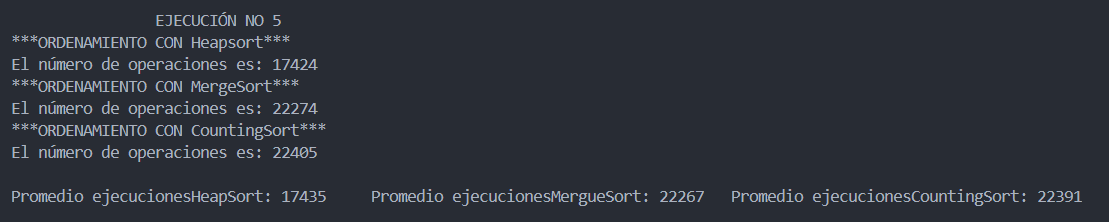
\includegraphics[width=16cm]{Images/Tam.800/2.png}
\par\vspace{0.4cm}
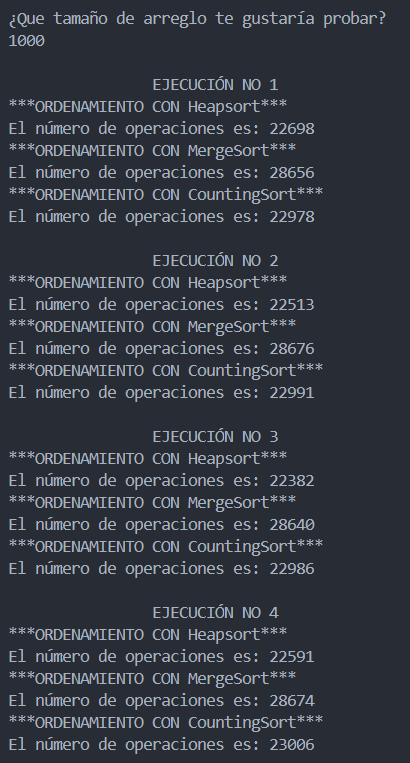
\includegraphics[width=9cm]{Images/Tam.1000/1.png}
\par\vspace{0.4cm}
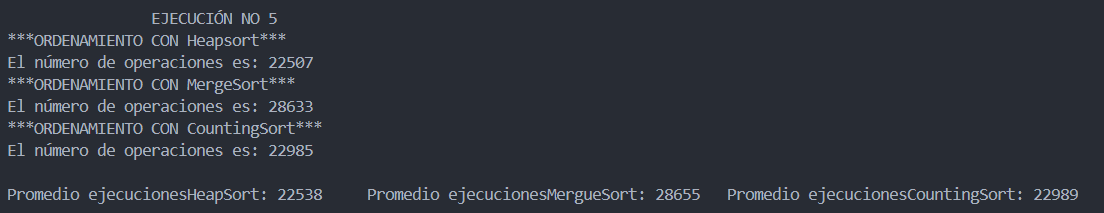
\includegraphics[width=16cm]{Images/Tam.1000/2.png}
\par\vspace{0.4cm}
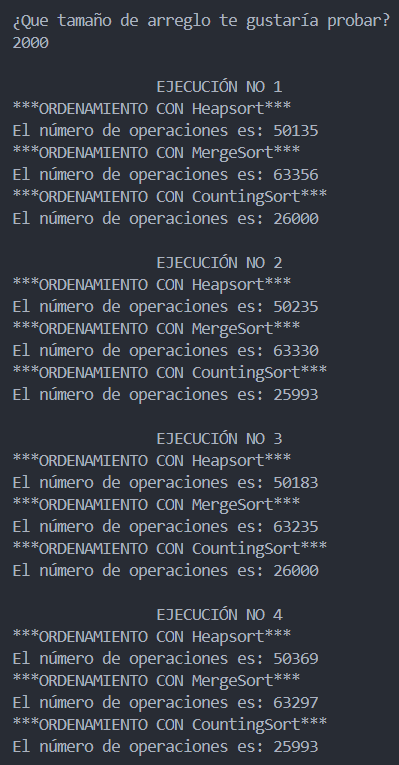
\includegraphics[width=9cm]{Images/Tam.2000/1.png}
\par\vspace{0.4cm}
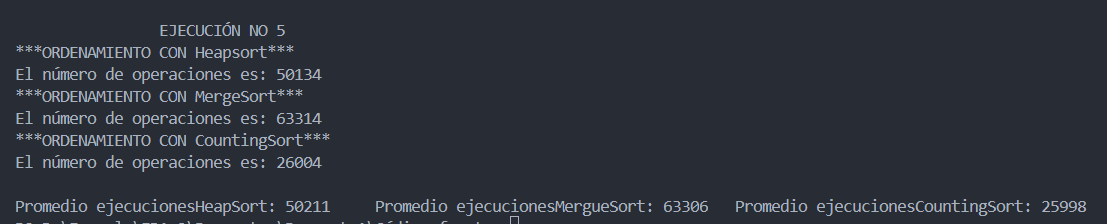
\includegraphics[width=16cm]{Images/Tam.2000/2.png}
\par\vspace{0.4cm}
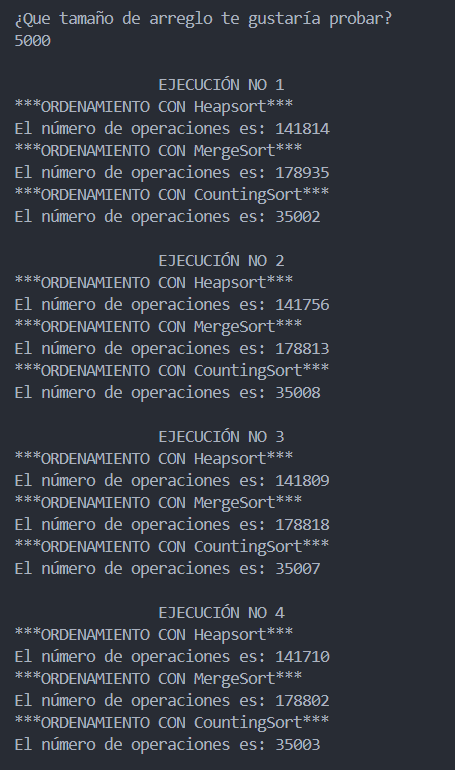
\includegraphics[width=9cm]{Images/Tam.5000/1.png}
\par\vspace{0.4cm}
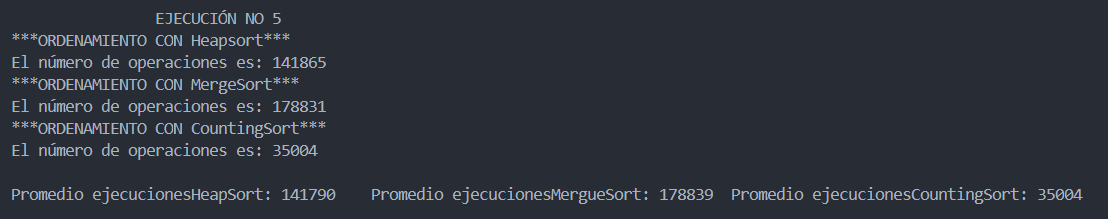
\includegraphics[width=16cm]{Images/Tam.5000/2.png}
\par\vspace{0.4cm}
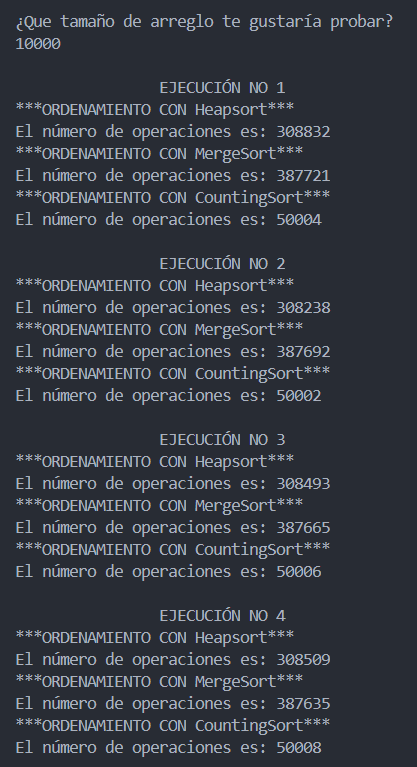
\includegraphics[width=9cm]{Images/Tam.10000/1.png}
\par\vspace{0.4cm}
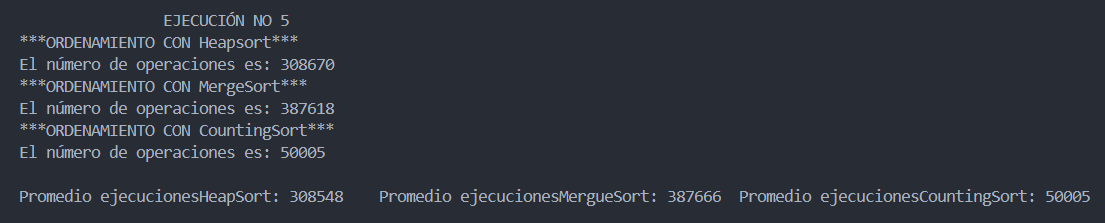
\includegraphics[width=16cm]{Images/Tam.10000/2.png}
\par\vspace{0.4cm}
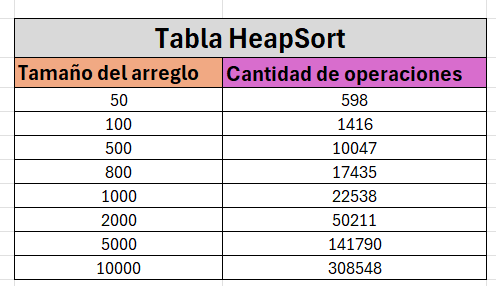
\includegraphics[width=15cm]{Images/Tab_HS.png}
\par\vspace{0.4cm}
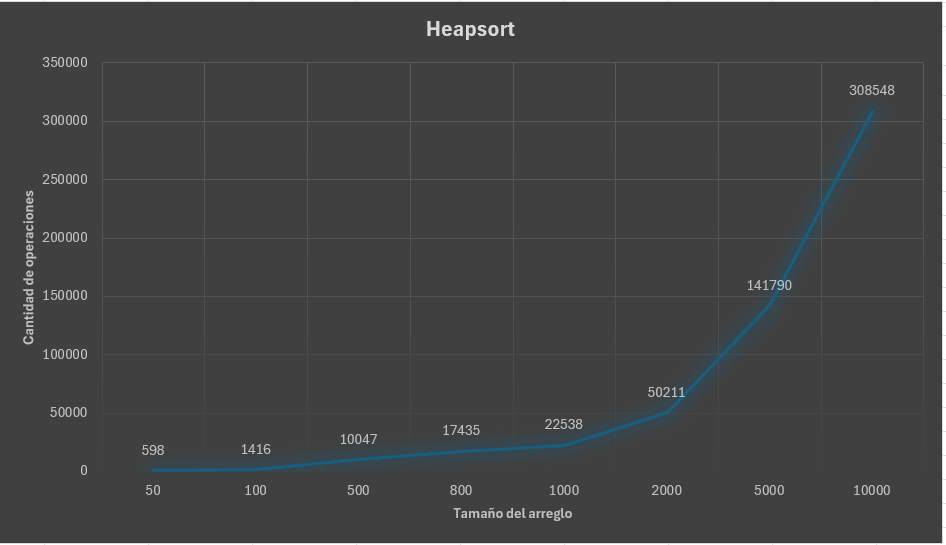
\includegraphics[width=15cm]{Images/Graf_HS.png}
\par\vspace{0.4cm}
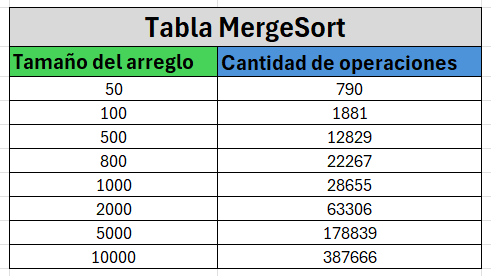
\includegraphics[width=15cm]{Images/Tab_MS.png}
\par\vspace{0.4cm}
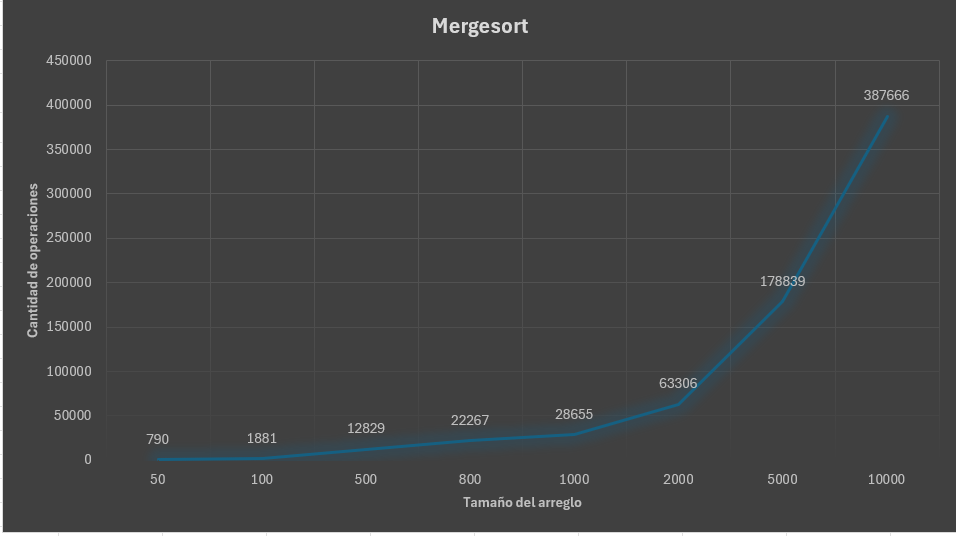
\includegraphics[width=15cm]{Images/Graf_MS.png}
\par\vspace{0.4cm}
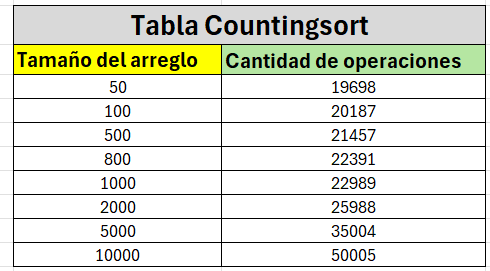
\includegraphics[width=15cm]{Images/Tab_CS.png}
\par\vspace{0.4cm}
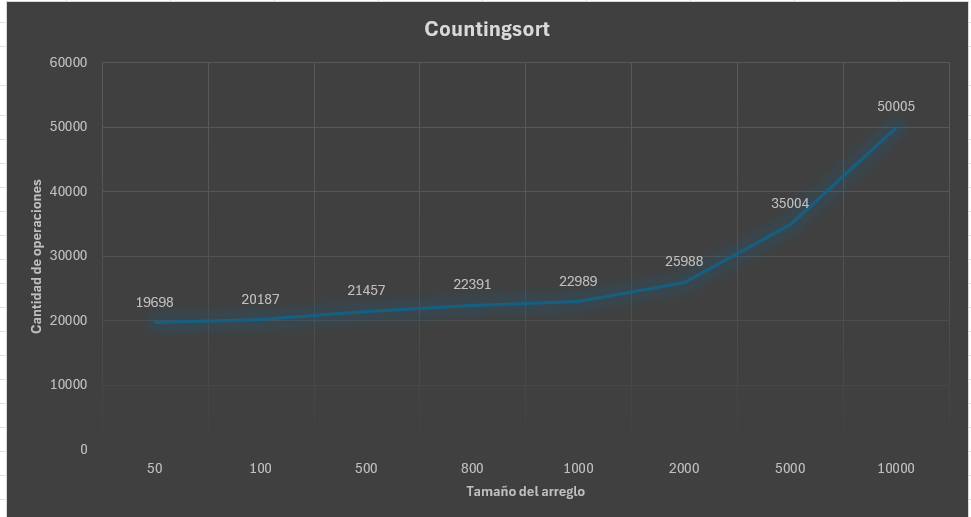
\includegraphics[width=15cm]{Images/Graf_CS.png}
\par\vspace{0.4cm}
Análisis Comparativo de Algoritmos de Ordenamiento
\par\vspace{0.4cm}
En el estudio exhaustivo de los algoritmos de ordenamiento, hemos observado patrones interesantes al comparar repetidamente MergeSort, HeapSort y CountingSort. Estas observaciones nos han proporcionado valiosas perspectivas sobre la eficiencia relativa de estos métodos.
\par\vspace{0.4cm}
\begin{enumerate}
    \item Disparidad en el Rendimiento
          \begin{itemize}
              \item Después de realizar múltiples ejecuciones con diferentes tamaños de arreglos, notamos una disparidad significativa en el número de operaciones realizadas por cada algoritmo.
              \item Específicamente, cuando superamos un rango de tamaño de arreglo (aproximadamente 1000 elementos), CountingSort se destaca como más eficiente en términos del número total de operaciones en comparación con los otros dos algoritmos.
          \end{itemize}
    \item El Dilema de los Datos Dispersos:
          \begin{itemize}
              \item Para comprender esta diferencia, consideremos un ejemplo concreto. Supongamos que tenemos una tabla de cinco elementos con datos que varían de 1000 a 9999.
              \item El arreglo original tiene solo cinco elementos, mientras que el arreglo de conteo abarca un rango mucho más amplio (de 1000 a 9999).
              \item Cuando el tamaño del arreglo a ordenar supera los 1000 elementos, notamos que el arreglo de conteo se ajusta gradualmente al tamaño del arreglo original. Esto se debe a la dispersión de los datos en el rango más amplio.
          \end{itemize}
    \item Complejidad de Operaciones y Tiempo:
          \begin{itemize}
              \item La complejidad de operaciones en CountingSort es similar a la complejidad de tiempo, expresada como O(n + k).
              \item Aquí, n representa el tamaño del arreglo original, y k es el rango de valores posibles. A medida que n aumenta, la influencia de k se vuelve más evidente.
          \end{itemize}
\end{enumerate}
\par\vspace{0.4cm}
Influencia de la Dispersión de Datos en los Algoritmos de Ordenamiento
\par\vspace{0.4cm}
En el análisis profundo de los algoritmos de ordenamiento, surge una reflexión importante: la dispersión de los datos ejerce una influencia significativa en la elección del método adecuado. Consideremos este aspecto con mayor detalle.
\par\vspace{0.4cm}
\begin{enumerate}
    \item Rango de Valores y Eficiencia:
          \begin{itemize}
              \item La variabilidad en los valores presentes en un conjunto de datos afecta directamente la eficiencia de los algoritmos de ordenamiento.
              \item En particular, cuando se trata de algoritmos como CountingSort, el rango de los números desempeña un papel crucial.
          \end{itemize}
    \item CountingSort y su Sensibilidad al Rango:
          \begin{itemize}
              \item CountingSort es altamente sensible al rango de valores. Su complejidad está directamente relacionada con la cantidad de valores únicos en el conjunto.
              \item Si el rango es pequeño (es decir, los valores están concentrados en un intervalo estrecho), CountingSort se vuelve más eficiente.
          \end{itemize}
    \item Comparación con Otros Algoritmos:
          \begin{itemize}
              \item En contraste, algoritmos como MergeSort y HeapSort no son tan sensibles al rango. Su complejidad depende principalmente del tamaño del arreglo (n).
              \item Cuando el rango es pequeño y se acerca a n, CountingSort supera a los otros algoritmos en términos de operaciones realizadas.
          \end{itemize}
\end{enumerate}
\par\vspace{0.4cm}
\textbf{En cuanto a QuickSort e InsertionSort:}
\par\vspace{0.4cm}
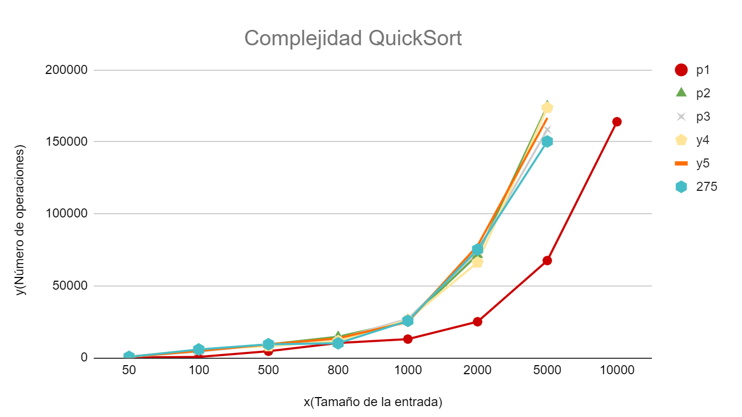
\includegraphics[width=15cm]{Images/Graf_QS.png}
\par\vspace{0.4cm}
Se realizaron 6 ejecuciones para analizar el algoritmo \texttt{quickSort}, el algoritmo \texttt{quickSort} tiene una complejidad para el mejor caso de $n \log n$, en la gráfica que se muestra se observa que la complejidad del algoritmo se tuvo para el mejor caso. Esto también se verificó manualmente; un ejemplo es que para la línea de color rojo que se muestra en la gráfica, la cantidad de operaciones realizadas para el arreglo de tamaño: $50$, $100$, $500$, $800$, $1000$, $2000$, $5000$ y $10000$, fueron los siguientes: $293$, $630$, $4561$, $10274$, $12999$, $25068$, $67554$, $163990$, estos resultados se encuentran dentro del rango de la complejidad $n\log n$ de cada tamaño del arreglo mencionado.
\par\vspace{0.4cm}
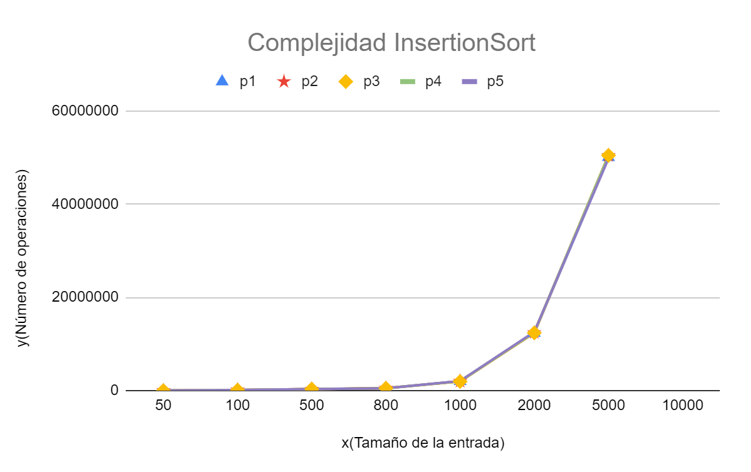
\includegraphics[width=15cm]{Images/Graf_IS.png}
\par\vspace{0.4cm}
El algoritmo \texttt{insertionSort} tiene una complejidad \( O(n) \) lineal, si el arreglo se encuentra ordenado ya que la única operación que realizaría serían comparaciones estas serían igual al tamaño del arreglo. Sin embargo, trabajamos con un arreglo desordenado por ello se tiene una complejidad cuadrada para el caso promedio y el peor caso; esto se puede observar en la gráfica donde también se comprobó manualmente y los resultados de las operaciones se encuentran dentro del rango de la complejidad cuadrada usando a cada tamaño del arreglo.
\par\vspace{0.6cm}
\textbf{En cuanto a SelectionSort y BubbleSort:}
EJECUCIONES:
\par\vspace{0.4cm}
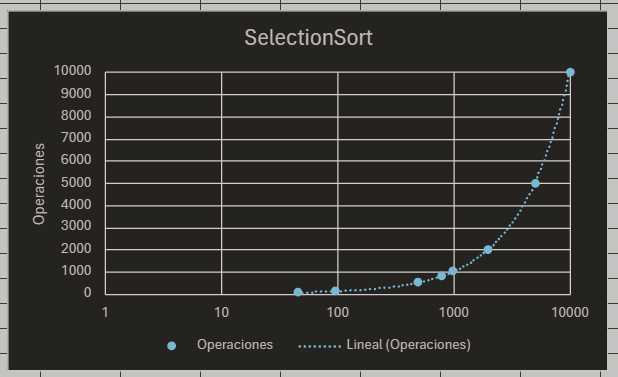
\includegraphics[width=15cm]{Images/Graf_SS.png}
\par\vspace{0.4cm}
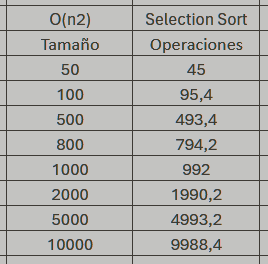
\includegraphics[width=15cm]{Images/Tab_SS.png}
\par\vspace{0.4cm}
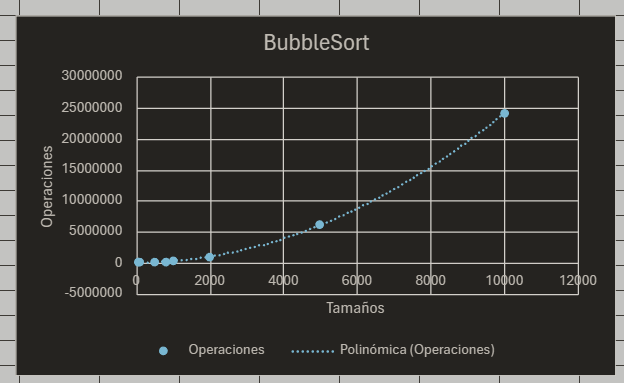
\includegraphics[width=15cm]{Images/Graf_BS.png}
\par\vspace{0.4cm}
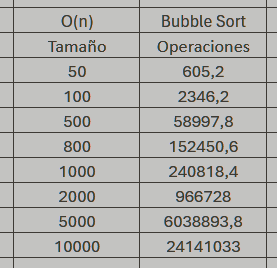
\includegraphics[width=15cm]{Images/Tab_BS.png}
\par\vspace{0.4cm}
Al verificar los resultados promedio de nuestras gráficas, podemos establecer que:
\begin{itemize}
  \item \textbf{SelectionSort} tiene una complejidad aproximada (dependiendo del mejor o peor caso) de \(O(n)\) a \(O(n^2)\) que tiende a ser más constante \(O(n^2)\) al aumentar el número de elementos del arreglo a ordenar.
  \item \textbf{BubbleSort} tiene una complejidad de \(O(n^2)\) que puede reducirse al ser modificada solo al momento de presentarse el mejor caso \(O(n)\).
\end{itemize}

\newpage
\textcolor{blue}{\textbf{CONCLUSIONES}}

\section{Quetzalli Zarate Menes}
\par\vspace{0.4cm}
Nuestro análisis imparcial nos ha permitido comprender las fortalezas y debilidades de cada algoritmo en diferentes contextos. CountingSort brilla en situaciones donde el rango de valores es amplio, mientras que MergeSort y HeapSort son más eficientes para arreglos más pequeños. La elección del algoritmo adecuado depende de las características específicas del problema y los datos involucrados.
\par\vspace{0.4cm}
En conclusión, la dispersión de datos es un factor clave al seleccionar el algoritmo de ordenamiento apropiado. CountingSort brilla cuando el rango es pequeño, mientras que MergeSort y HeapSort son más versátiles en una variedad de situaciones.
\par\vspace{0.7cm}
¿Quien gana QuickSort, HeapSort o MergeSort?
\par\vspace{0.4cm}
QuickSort es mejor en muchos escenarios prácticos por varias razones:
\par\vspace{0.4cm}
Constantes pequeñas: En la práctica, las constantes involucradas en la complejidad de QuickSort son menores en comparación con otros algoritmos ( O(n log n) ), lo que significa que en conjuntos de datos típicos, QuickSort será más rápido.
\par\vspace{0.4cm}
La superioridad de QuickSort sobre HeapSort puede atribuirse a su mayor eficiencia en la realización de intercambios. QuickSort, mediante su estrategia de partición, asigna a cada elemento su posición definitiva en un solo movimiento, lo que resulta en una menor cantidad de intercambios totales. Por otro lado, HeapSort requiere reajustes constantes del montículo (heap) después de cada eliminación de la raíz, lo que incrementa el número de operaciones necesarias. Además, en el análisis del caso promedio, QuickSort tiende a realizar menos intercambios en comparación con HeapSort, lo que contribuye a su eficacia general y lo convierte en una opción preferente para la ordenación de datos.
\par\vspace{0.6cm}
\section{López Martínez Diana}
\begin{itemize}
    \item El algoritmo \texttt{quickSort} demostró tener una complejidad temporal óptima en el mejor caso de $n \log n$, lo cual fue evidenciado tanto por la experimentación como por el análisis manual. Los resultados obtenidos para diferentes tamaños de arreglos se alinearon con la complejidad teórica esperada.
    \item Para el algoritmo \texttt{insertionSort}, se observó que su comportamiento es lineal $O(n)$ cuando el arreglo está previamente ordenado, limitándose a realizar comparaciones. No obstante, en arreglos desordenados, la complejidad se eleva a cuadrática, como se refleja en los resultados experimentales y el análisis manual.
    \item Las modificaciones realizadas para incluir contadores de operaciones en ambos algoritmos permitieron un análisis detallado de su complejidad. La implementación de un método para reiniciar los contadores resultó ser una solución inicial; sin embargo, la inicialización de los contadores en cero desde el comienzo eliminó la necesidad de reiniciarlos y resolvió el problema de acumulación de operaciones.
  \end{itemize}
  \par\vspace{0.6cm}
\section{Giron Escalona Erendira Nayely}
Al registrar el número de veces que se realizan operaciones durante la ejecución de un algoritmo, obtenemos una mejor comprensión de su comportamiento en diferentes escenarios y podemos compararlo con otros algoritmos de ordenamiento para determinar su eficacia en términos de tiempo y recursos utilizados.
\par\vspace{0.4cm}
Los algoritmos de ordenamiento \textbf{Selection Sort} y \textbf{Bubble Sort}  presentan diferentes enfoques y eficiencia en términos de complejidad. \textbf{Selection Sort}, aunque simple de entender e implementar, tiene una complejidad cuadrática en el peor de los casos (\(O(n^2)\)), lo que lo hace menos eficiente para conjuntos de datos grandes. Por otro lado, \textbf{Bubble Sort} también tiene una complejidad cuadrática, pero su característica de comparación adyacente puede ser ineficiente, especialmente en arreglos casi ordenados. Ambos algoritmos son adecuados para pequeñas cantidades de datos o como ejemplos introductorios de algoritmos de ordenamiento.
\par\vspace{1cm}
\newpage
\begin{thebibliography}{9}
    \bibitem{cormen} 
    Cormen, T. H., Leiserson, C. E., Rivest, R. L., \& Stein, C. (2009). 
    \textit{Algoritmos: Teoría y práctica} (3a ed.). 
    McGraw-Hill Interamericana.
    
    \bibitem{baase} 
    Baase, S., \& Van Gelder, A. (2002). 
    \textit{Algoritmos computacionales: introducción al análisis y diseño}.
    
    \bibitem{drozdek} 
    Drozdek, A. (2007). 
    \textit{Estructuras de datos y algoritmos con Java}. 
    Cengage Learning Mexico.
    
    \bibitem{sierra} 
    Sierra, F. J. C. (2019). 
    \textit{C/C++: curso de programación}.
    
    \bibitem{afteracademy} 
    Comparación de algoritmos de clasificación. (20 de febrero de 2024). 
    AfterAcademy. 
    \texttt{https://afteracademy.com/blog/comparison-of-sorting-algorithms}
    \end{thebibliography}

\end{document}